\documentclass[a4paper,lang=cn,10pt,newtx,scheme=chinese]{elegantbook}

\iffalse
\title{ElegantBook:优美的 \LaTeX{} 书籍模板}
\subtitle{Elegant\LaTeX{} 经典之作}

\author{Ethan Deng \& Liam Huang}
\institute{Elegant\LaTeX{} Program}
\date{Aug 17, 2022}
\version{4.5}
\bioinfo{自定义}{信息}

\extrainfo{要让一群人团结起来,需要的不是英明的领导,而是共同的敌人。—— 比企谷八幡}

\setcounter{tocdepth}{3}

\logo{logo-blue.png}
\fi
%\begin{titlepage}
%\cover{figure/cover.jpg}
\cover{Bilder/Front_Cover_.png}
%\end{titlepage}

% 本文档命令
\usepackage{array}
\newcommand{\ccr}[1]{\makecell{{\color{#1}\rule{1cm}{1cm}}}}

% 修改标题页的橙色带
\definecolor{customcolor}{RGB}{32,178,170}
\colorlet{coverlinecolor}{customcolor}
\usepackage{cprotect}

\addbibresource[location=local]{reference.bib} % 参考文献,不要删除

\begin{document}

\maketitle
\frontmatter

\tableofcontents

\mainmatter

\part{Aachen 及周边}

%!TEX root = ../hcwsa_.tex

\chapter{亚琛概况}

\section{亚琛市}

\href{https://www.aachen.de/CHIN/kurzinfo.html}{\textsbf{亚琛/Aachen}}\footnote{亚琛市网站有汉语介绍。} ,是德国\href{https://www.land.nrw/en/welcome}{\textsbf{北莱茵-威斯特法伦州/北威州/Nordrhein-Westfalen/North Rhine-Westphalia}}\footnote{北威州网站有英语、德语和荷兰语三种语言介绍。}的一个边陲城市,她位于欧洲的中心,地处德国、荷兰和比利时三国交界处。因为地理位置的原因,亚琛也是一个非常重要的铁路汇集点,同时也是工业汇集中心,素有 ”欧洲心脏”之称。

亚琛拥有众多大学和科研机构,其中最负盛名的学校当属亚琛工业大学。亚琛工业大学吸引了约三万一千名学子来此学习深造。通过校方和当地学者的努力,亚琛在过去的几年中顺利完成了地区结构转型。汽车工程、激光技术、微芯片结构及医学领域的研究,让这个曾经的矿工业区变成了如今的高科技基地。高等专科学校和音乐学院也让大学生的总人数上升至四万人。与此同时,还有很多参加专业会议、学术交流的专家和学者经常来到亚琛。欧洲国会中心也为到访者提供了多功能的会议场所。年轻人的加入给这座古老的城市注入了生机和年轻的血液,也它也焕发出青春的活力。

\section{亚琛工业大学}

\href{https://www.rwth-aachen.de/go/id/a/?lidx=1}{\textsbf{亚琛工业大学/Rheinisch-Westfälische Technische Hochschule Aachen/RWTH Aachen}},创建于1870年,是位于德国亚琛的世界顶尖理工类大学,世界百强大学。其在工科领域享有极高的声誉,是欧洲顶尖理工大学IDEA联盟成员之一。

亚琛工业大学现为11所德国精英大学 (Exzellenzinitiative) 之一、9所顶尖德国理工大学联盟 (TU9) 成员之一。其同时是TIME欧洲顶尖工业管理者高校联盟、CESAER欧洲高等工程教育和研究大学会议联盟、PEGASUS欧洲航空航天大学联盟等一系列组织成员。

顶尖的科研与教育水平让许多著名公司如微软、福特、爱立信、飞利浦、联合技术等都在亚琛建立了分部,三菱则在附近建立了欧洲半导体中心。亚琛工业大学的校友出众,学术界有钱学森的导师冯·卡门,工业界有西门子、保时捷、宝马、奥迪、宾利等企业总裁。前中国科学院院长路甬祥、教育部副部长韦钰、原清华大学校长王大中也毕业于该校。

学校自创建以来产生过6位诺贝尔奖得主,10位莱布尼茨奖得主。学校尤其重视国际化合作,是从工业和企业界获得最多经费的德国大学。

\section{亚琛应用科技大学}

\href{https://www.fh-aachen.de/}{\textsbf{亚琛应用科技大学/Fachhochschulen Aachen - Aachen University of Applied Sciences/FH Aachen}}成立于1971年,是德国著名的应用科技大学之一。该校由多所应用技术大学和职业培训中心合并而成,100多年来落实以实践为导向的教育传统,在电气、机械工程、信息学等应用科学领域名列德国第一。

在研究方面,亚琛应用科技大学力争成为德国最强大的应用技术大学之一。能力主要是在未来的能源、移动和生命科学领域。最新的研究成果直接纳入教学。其机械工程和机电一体化在全德同类大学 (应用科技大学或高等专科学校) 中排名第一位。

\section{亚琛语言学院}

在德语作为外语 (DaF) 领域,\href{https://www.spraachen.org/}{\textsbf{亚琛语言学院}}作为地区最大的语言学院,开设全面的强化及备考课程,涵盖德语水平等级A1至C1,为每年不断增多的有学术背景的德语学习者服务:大学申请人,大学生,硕博研究生,已完成培训的学者以及在职人员是该校课程主要面向的群体。作为官方认证的考试中心,该校定期举办各类标准化语言考试。

几年前分布亚琛各地的亚琛语言学院各专业部门于2011年一起搬进坐落于亚琛市中心的Haus der Kohle。亚琛语言学院以德国为中心现设有以下三处办公地点:亚琛,于利希,以及北京 (中国分部)。

\section{于利希研究中心}

\href{https://www.fz-juelich.de/portal/DE/Home/home_node.html}{\textsbf{于利希研究中心/Jülich Forschungszentrum/FZJ}}是德国亥姆霍兹国家研究中心联合会的下属科研机构,主要从事物质结构、能源、信息、生命、环境和运输航天等方向的研究。现有超过5000名研究人员,是欧洲最大的科学研究机构之一。

研究中心在核物理、磁共振脑成像、太阳能电池和高倍透射电镜等方面的研究处于世界前沿。其中固体研究所Peter Grünberg 教授因发现巨磁电阻效应而荣获2007年诺贝尔物理学奖。
于利希研究中心与亚琛工业大学成立了\href{https://www.jara.org/en/}{\textsbf{Jülich-Aachen研究联盟/JARA}},多年来吸引了RWTH的众多毕业生到FZJ从事博士课题研究。

\chapter{当地组织}

\section{中国驻杜塞尔多夫总领馆}


\section{RWTH 的职能部门}

\section{亚琛中国学生学者联合会}

\section{亚琛中德协会}

\section{各类学生社团}


\part{初来乍到}

%!TEX root = ../hcwsa.tex

\chapter{银行}

外籍学生都必须使用德国境内的银行进行消费,它是申请德国签证必需的材料之一;此外,银行的选择涉及到在当地消费的便捷度。

为使概念明晰,我们把银行的\textsbf{开户}和\textsbf{激活}都放在这里介绍,尽管激活是入境后才需要去办的事情。

\section{概念澄清}
 
目前亚琛有两家较大的银行支持在国内办理\textsbf{开户/Account Opening},分别是\href{https://www.deutsche-bank.de/pk.html}{\textsbf{德意志银行/德银/Deutsche Bank/DB}}和\href{https://www.sparkasse-aachen.de/de/home.html}{\textsbf{亚琛储蓄银行/Sparkasse Aachen/Sparkasse}}。后文用德银和Sparkasse指代。

用于\textbf{申请德国签证}所开通的德国境内的银行账户是指\textsbf{冻结账户/Blocked Account/Sperrkonto},存入的资金叫\textsbf{冻结资金/Blocked Balance/Sperrbetrag}。词缀\textsbf{冻结/Blocked/Sperr-}指的是开户人在前往开户行所在国(德国)之前\textbf{不得使用}该账户内的资金,这是各国银行出于涉外金融安全的考虑而做的举措。类似字样也出现于签证相关的文件里的 “冻结” 和 “解冻”。开户会涉及到\textbf{手续费} (含信件运费),通常是150欧左右。

用于\textbf{在德国当地消费}的银行账户称为\textsbf{借记账户/Debit Account/Girokonto}。在到达了亚琛、有了固定地址、办理了\textsbf{Anmelden的证明}以后,即可办理Sperrkonto和Girokonto的激活手续。

用于日常消费 (如支付房租) 的银行卡是指Girokonto的\textsbf{借记卡/储蓄卡/Debit Card/Girocard}及其IBAN。Sperrkonto是不发卡的。

每一个留德学生的名下都有Sperrkonto和Girokonto。这两个账户的关系是:\textbf{Sperrkonto每月自动把一定数额的欧元(853欧)汇入到Girokonto}。关于这两个账户跟德银和Sparkasse的区别见Table.1。

\textsbf{冻结账户/Sperrkonto}是被提款的,因此它也被称为\textsbf{限制提款账户} (这出现在签证文件的用词里)。\textsbf{冻结资金}也称\textsbf{自保金},每月提款额度不得超过一定金额,如853欧。所规定的这853欧是最基本的生活保障,是为了保障留德学生有足够的资金维持在当地一年共计10,236欧的生活费用\footnote{当然,您还可以通过其他方式获得更多的生活费。所以853欧并不是固定的,在开户表格上可以自行决定。}。这个数额是德国政府基于在德大学生的消费调查而规定的,相对稳定,不随利率波动\footnote{2018年的自保金数额是8,640欧,这个数额已沿用多年,而2020年的数额则是10,236欧。}。

Fig.1是两个银行的卡的样例。欧盟的银行系统里对\textsbf{账户号/Konto-Nr/IBAN}和\textsbf{卡号/Karten-Nr}是有区分的。\textsbf{Karten-Nr}的具体格式取决于银行。这种设计是为了防止卡遗失\footnote{挂失后新发的卡的Karten-Nr跟旧卡的Karten-Nr不一样,但他们的IBAN是一样的。}。

银行系统有\textsbf{借记卡/储蓄卡/Debit Card/Girocard} (不可透支) 和\textsbf{贷记卡/信用卡/Kreditkarte} (可透支) 两种类型的账户的区分。借记卡和贷记卡是书面语,储蓄卡和信用卡是口语。由于货币的结算方式不同,银行规定,借记卡只能用于发卡行的境内消费,而贷记卡则可以用于国际消费,以特定的结算方式计入到发卡行所在国的持卡人的借记卡上。\textsbf{银联/UnionPay}、\textsbf{VISA}、\textsbf{MasterCard/万事达}是不同贷记卡所采用的不同的结算方式。Sparkasse在信用卡的业务上推行了不少福利,在办理Girokonto激活业务的同时会推荐办理其贷记卡。

\begin{table}[h]
\centering
\caption{title}
\begin{tabular}{|c|c|c|}
\hline
&Sperrkonto&Girokonto\\
\hline
德银&\multicolumn{2}{c|}{同一个IBAN}\\
\hline
Sparkasse&IBAN for Sperrkonto&IBAN for Girokonto\\
\hline
\end{tabular}
\end{table}

下面分别讲述德银和Sparkasse的开户和激活流程。

\section{德意志银行}

德意志银行的开户流程如这里所示:

\begin{enumerate}
  \item 从官网下载申请表格并且填写。默认853欧的每月提款额度可以填写其他数额。
  \item 前往德银驻北/上/广分行办理相关材料,并将拿到个人编号通知单。
  \item 根据个人编号通知单的信息汇款。该通知单上有两个收款账号:一个是德银总部的负责相关业务部门的IBAN,汇款的8640欧是自保金;另一个是 德银驻华分行的工作人员的账号,汇的是手续费。
  \item 先后收到来自德银驻北/上/广分行的两份纸质信函,分别是存款证明和开户证明/Kontoeröffnung。后者有您的IBAN。
\end{enumerate}

至此,德银的开户流程办理完毕。下面是激活流程:

\begin{enumerate}
  \setcounter{enumi}{4}
  \item Anmelden,得到相关的证明,上面有您在德国的长期住址。
  \item 在官网->Activate a blocked account下载表格填写,打印,签字。街头的打印店有unicopy。
  \item 邮寄给汉堡办事处,网上搜索\textsbf{Deutsche Post}可知邮筒的位置。不必去\textsbf{德银驻亚琛支行/Deutsche Bank Filiale Aachen}。
  \item 大约一周以后,您会收到来自德银的若干封\textbf{纸质信件},包括但不限于网银密码、Girocard和卡密码、photoTAN (德国版的网银支付二维码),等等。
\end{enumerate}

\section{Sparkasse Aachen}

  Sparkasse Aachen的办理流程如这里所示,实际上发邮件即可:

  \begin{enumerate}
    \item 根据如下模板发邮件给 896-visa@sparkasse-aachen.de 告知银行的工作人员说您要开通Sperrkonto。附件为\textbf{大学录取通知书}和\textbf{护照}。
  \end{enumerate}

  \noindent\fbox{
    \begin{minipage}{\textwidth}
    Betreff: Sperrkonto/ blocked account

    Sehr geehrte Damen, sehr geehrte Herren,

    Dear Sir or Madam,

    \vskip1em

    Als zukunftige Studentin einer Hochschule in Aachen mochte ich bei der Sparkasse Aachen ein Sperrkonto einrichten.

    As a future student at one of the universities in Aachen, I would like to create a blocked account at Sparkasse Aachen.

    \vskip1em

    Die Bestatigung liber den Studienplatz der Hochschule und eine Passkopie habe ich als Emailanhang beigefiigt.

    The confirmation of acceptance at the university and the passport copy is attached.

    \vskip1em

    Viele GruBe

    Kind regards

    Vorname Nachname
    \end{minipage}
  }

  \begin{enumerate}
    \setcounter{enumi}{1}
    \item 工作人员回复,让您汇款给Sparkasse的账户,以及提供您的地址和电话等资料。 
    \item 收到存款证明和开户证明/Kontoeröffnung这两个文件的纸质信函和Email。
  \end{enumerate}

  至此,Sparkasse的开户流程办理完毕。下面是激活流程:

  \begin{enumerate}
    \setcounter{enumi}{3}
    \item Anmelden,得到相关的证明,上面有您在德国的长期住址。
    \item 打电话约Termin,届时带上护照和Anmelden的证明前往Sparkasse Aachen Filiale办理Sperrkonto的激活以及Girokonto的开户和激活。在Girokonto的开户表格上确定每月提款额度。
    \item 收到网银密码、Girocard和卡密码。
  \end{enumerate}

\section{两家银行的对比}

  经过上述步骤即可在银行或者通过ATM机自助取款了\footnote{Sperrkonto 激活激活之前也可以用国内的\textbf{银联卡}在 ATM 机取款,是根据实时汇率从人民币扣款的。}。Sparkasse Aachen在全亚琛有大大小小的ATM机以及银行服务点,取钱和办理各种银行服务较为方便。而德银的冻结资金办理手续比较繁琐,且其ATM机在亚琛的分布相对较少。

  Sparkasse Aachen提供的Girokonto服务比较多样,如\href{https://www.sparkasse-aachen.de/de/home/privatkunden/girokonto/s-pool.html}{\textsbf{S-POOL Konto}}。这是Sparkasse Aachen专门为18-30岁的学生准备的青年账户。只需要出示有效的学生证明,办理S-POOL Konto的账户时即可享受优惠的账户管理费。办理S-POOL账户时,还可以选择免费申请一张Mastercard,对于买机票住酒店等大额消费来说非常的方便。此外,S-POOL 账户还和亚琛的诸多商家有合作,付款时使用S-POOL卡能够享受优惠。

  因此相较来讲,Sparkasse Aachen是在亚琛学习和生活的首选。

\chapter{医疗保险}

\section{私保申请和缴费}

\section{公保申请}

\section{ElegantBook 写作示例}

\begin{introduction}
  \item 积分定义~\ref{def:int}
  \item Fubini 定理~\ref{thm:fubi}
  \item 最优性原理~\ref{pro:max}
  \item 柯西列性质~\ref{property:cauchy}
  \item 韦达定理
\end{introduction}

\section{Lebesgue 积分}
在前面各章做了必要的准备后,本章开始介绍新的积分。在 Lebesgue 测度理论的基础上建立了 Lebesgue 积分,其被积函数和积分域更一般,可以对有界函数和无界函数统一处理。正是由于 Lebesgue 积分的这些特点,使得 Lebesgue 积分比 Riemann 积分具有在更一般条件下的极限定理和累次积分交换积分顺序的定理,这使得 Lebesgue 积分不仅在理论上更完善,而且在计算上更灵活有效。

Lebesgue 积分有几种不同的定义方式。我们将采用逐步定义非负简单函数,非负可测函数和一般可测函数积分的方式。

由于现代数学的许多分支如概率论、泛函分析、调和分析等常常用到一般空间上的测度与积分理论,在本章最后一节将介绍一般的测度空间上的积分。

\subsection{积分的定义}

我们将通过三个步骤定义可测函数的积分。首先定义非负简单函数的积分。以下设 $E$ 是 $\mathcal{R}^n$ 中的可测集。

\begin{definition}[可积性] \label{def:int} 
设 $ f(x)=\sum\limits_{i=1}^{k} a_i \chi_{A_i}(x)$ 是 $E$ 上的\textbf{非负简单函数},中文其中 $\{A_1,A_2,\ldots,A_k\}$ 是 $E$ 上的一个可测分割,$a_1,a_2,\ldots,a_k$ 是非负实数。定义 $f$ 在 $E$ 上的积分为 $\int_{a}^b f(x)$
\begin{equation}
   \label{inter}
   \int_{E} f dx = \sum_{i=1}^k a_i m(A_i) \pi \alpha\beta\sigma\gamma\nu\xi\epsilon\varepsilon. \oint_{a}^b\ointop_{a}^b\prod_{i=1}^n
\end{equation}
一般情况下 $0 \leq \int_{E} f dx \leq \infty$。若 $\int_{E} f dx < \infty$,则称 $f$ 在 $E$ 上可积。
\end{definition}

一个自然的问题是,Lebesgue 积分与我们所熟悉的 Riemann 积分有什么联系和区别?在 4.4 在我们将详细讨论 Riemann 积分与 Lebesgue 积分的关系。这里只看一个简单的例子。设 $D(x)$ 是区间 $[0,1]$ 上的 Dirichlet 函数。即 $D(x)=\chi_{Q_0}(x)$,其中 $Q_0$ 表示 $[0,1]$ 中的有理数的全体。根据非负简单函数积分的定义,$D(x)$ 在 $[0,1]$ 上的 Lebesgue 积分为
\begin{equation}
   \label{inter2}
   \int_0^1 D(x)dx = \int_0^1 \chi_{Q_0} (x) dx = m(Q_0) = 0
\end{equation}
即 $D(x)$ 在 $[0,1]$ 上是 Lebesgue 可积的并且积分值为零。但 $D(x)$ 在 $[0,1]$ 上不是 Riemann 可积的。


有界变差函数是与单调函数有密切联系的一类函数。有界变差函数可以表示为两个单调递增函数之差。与单调函数一样,有界变差函数几乎处处可导。与单调函数不同,有界变差函数类对线性运算是封闭的,它们构成一线空间。练习题 \ref{exer:43} 是一个性质的证明。

\begin{exercise}\label{exer:43}
设 $f \notin\in L(\mathcal{R}^1)$,$g$ 是 $\mathcal{R}^1$ 上的有界可测函数。证明函数
\begin{equation}
   \label{ex:1}
   I(t) = \int_{\mathcal{R}^1} f(x+t)g(x)dx \quad t \in \mathcal{R}^1
\end{equation}
是 $\mathcal{R}^1$ 上的连续函数。 
\end{exercise}

\begin{solution}
即 $D(x)$ 在 $[0,1]$ 上是 Lebesgue 可积的并且积分值为零。但 $D(x)$ 在 $[0,1]$ 上不是 Riemann 可积的。
\end{solution}

\begin{proof}
即 $D(x)$ 在 $[0,1]$ 上是 Lebesgue 可积的并且积分值为零。但 $D(x)$ 在 $[0,1]$ 上不是 Riemann 可积的。
\end{proof}

\begin{theorem}[Fubini 定理] \label{thm:fubi} 
(1)若 $f(x,y)$ 是 $\mathcal{R}^p\times\mathcal{R}^q$ 上的非负可测函数,则对几乎处处的 $x\in \mathcal{R}^p$,$f(x,y)$ 作为 $y$ 的函数是 $\mathcal{R}^q$ 上的非负可测函数,$g(x)=\int_{\mathcal{R}^q}f(x,y) dy$ 是 $\mathcal{R}^p$ 上的非负可测函数。并且
\begin{equation}
   \label{eq:461}
   \int_{\mathcal{R}^p\times\mathcal{R}^q} f(x,y) dxdy=\int_{\mathcal{R}^p}\left(\int_{\mathcal{R}^q}f(x,y)dy\right)dx.
\end{equation}

(2)若 $f(x,y)$ 是 $\mathcal{R}^p\times\mathcal{R}^q$ 上的可积函数,则对几乎处处的 $x\in\mathcal{R}^p$,$f(x,y)$ 作为 $y$ 的函数是 $\mathcal{R}^q$ 上的可积函数,并且 $g(x)=\int_{\mathcal{R}^q}f(x,y) dy$ 是 $\mathcal{R}^p$ 上的可积函数。而且~\eqref{eq:461} 成立。
\end{theorem}

\ref{thm:fubi}

\begin{note}
在本模板中,引理(lemma),推论(corollary)的样式和定理~\ref{thm:fubi} 的样式一致,包括颜色,仅仅只有计数器的设置不一样。
\end{note}

我们说一个实变或者复变量的实值或者复值函数是在区间上平方可积的,如果其绝对值的平方在该区间上的积分是有限的。所有在勒贝格积分意义下平方可积的可测函数构成一个希尔伯特空间,也就是所谓的 $L^2$ 空间,几乎处处相等的函数归为同一等价类。形式上,$L^2$ 是平方可积函数的空间和几乎处处为 0 的函数空间的商空间。

\begin{proposition}[最优性原理] \label{pro:max}
如果 $u^*$ 在 $[s,T]$ 上为最优解,则 $u^*$ 在 $[s, T]$ 任意子区间都是最优解,假设区间为 $[t_0, t_1]$ 的最优解为 $u^*$ ,则 $u(t_0)=u^{*}(t_0)$,即初始条件必须还是在 $u^*$ 上。
\end{proposition}

我们知道最小二乘法可以用来处理一组数据,可以从一组测定的数据中寻求变量之间的依赖关系,这种函数关系称为经验公式。本课题将介绍最小二乘法的精确定义及如何寻求点与点之间近似成线性关系时的经验公式。假定实验测得变量之间的 $n$ 个数据,则在平面上,可以得到 $n$ 个点,这种图形称为 “散点图”,从图中可以粗略看出这些点大致散落在某直线近旁, 我们认为其近似为一线性函数,下面介绍求解步骤。

\begin{figure}[htbp]
  \centering
  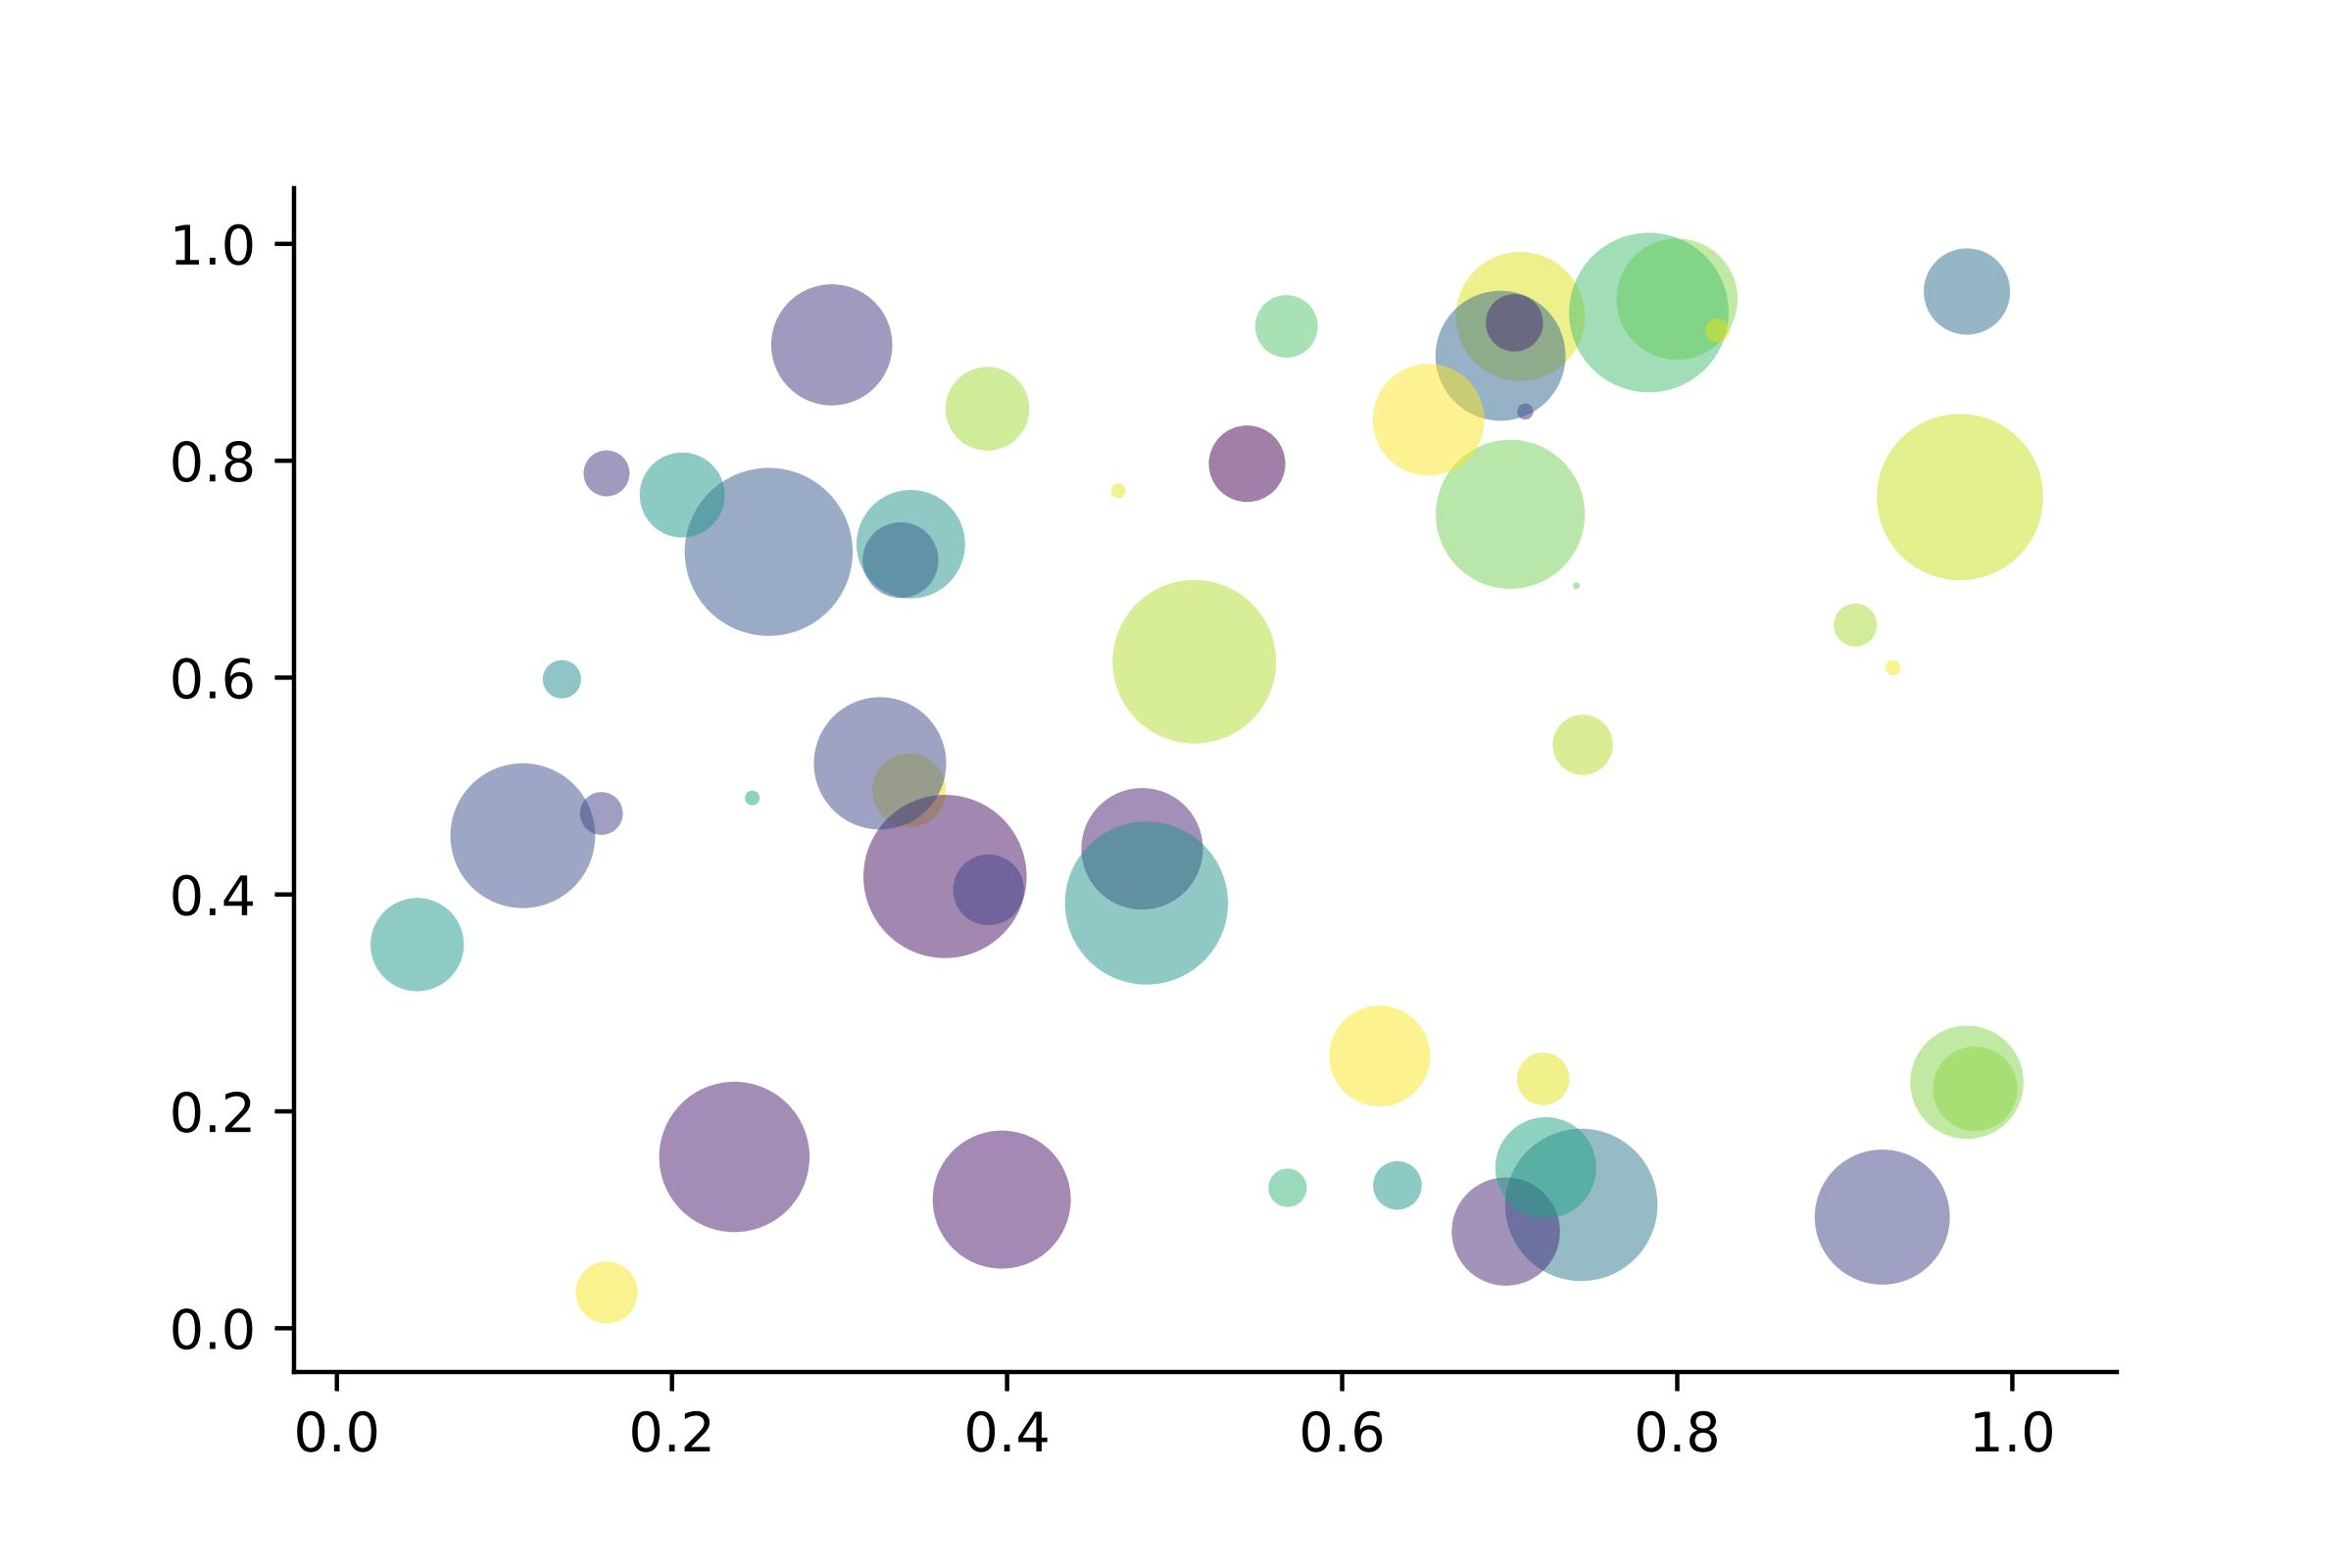
\includegraphics[width=0.6\textwidth]{scatter.jpg}
  \caption{散点图示例 $\hat{y}=a+bx$ \label{fig:scatter}}
\end{figure}

以最简单的一元线性模型来解释最小二乘法。什么是一元线性模型呢?监督学习中,如果预测的变量是离散的,我们称其为分类(如决策树,支持向量机等),如果预测的变量是连续的,我们称其为回归。回归分析中,如果只包括一个自变量和一个因变量,且二者的关系可用一条直线近似表示,这种回归分析称为一元线性回归分析。如果回归分析中包括两个或两个以上的自变量,且因变量和自变量之间是线性关系,则称为多元线性回归分析。对于二维空间线性是一条直线;对于三维空间线性是一个平面,对于多维空间线性是一个超平面。

\begin{property}\label{property:cauchy}
柯西列的性质
\begin{enumerate}
\item $\{x_k\}$ 是柯西列,则其子列 $\{x_k^i\}$ 也是柯西列。
\item $x_k\in \mathcal{R}^n$,$\rho(x,y)$ 是欧几里得空间,则柯西列收敛,$(\mathcal{R}^n,\rho)$ 空间是完备的。
\end{enumerate}
\end{property}

\begin{conclusion}
回归分析(regression analysis) 是确定两种或两种以上变量间相互依赖的定量关系的一种统计分析方法。运用十分广泛,回归分析按照涉及的变量的多少,分为一元回归和多元回归分析;按照因变量的多少,可分为简单回归分析和多重回归分析;按照自变量和因变量之间的关系类型,可分为线性回归分析和非线性回归分析。
\end{conclusion}

\begin{problemset}
\item 设 $A$ 为数域 $K$ 上的 $n$ 级矩阵。证明:如果 $K^n$ 中任意非零列向量都是 $A$ 的特征向量,则 $A$ 一定是数量矩阵。
\item 证明:不为零矩阵的幂零矩阵不能对角化。
\item 设 $A = (a_{ij})$ 是数域 $K$ 上的一个 $n$ 级上三角矩阵,证明:如果 $a_{11} = a_{22} = \cdots = a_{nn}$,并且至少有一个 $a_{kl} \not = 0 (k < l)$,则 $A$ 一定不能对角化。
\end{problemset}

\chapter{住房}

\section{住房形式}

\section{租房信息}

\section{租房合同和注意事项}

\section{租房广告里的常见名词之定义}

\section{出境前寻找住房的注意事项}

\chapter{申请签证及入境}

\section{签证申请}

\section{购买机票及入境}

\section{从入境城市乘坐列车到达亚琛}

\section{从车站乘公交到住所}

\chapter{重要事务办事点}

\section{市政厅}

\section{SuperC}

\section{外管局}
\chapter{入境两周内必办事宜}

\section{电话卡和宽带}

\section{签订住房合同以及 Anmelden}

\section{银行账户激活}

\section{医保激活}

\chapter{RWTH注册和管理系统}

\section{入学注册}

\section{学生管理系统}

\section{学生邮箱}
\chapter{延签和居留许可}

\section{申请}



\part{在亚琛学习和生活}

\chapter{学习、实习和科研}

\section{学期注册}

\section{选课和考试报名}

\section{自习室}

\nocite{*}

\printbibliography[heading=bibintoc, title=\ebibname]
\appendix

\begin{titlepage}
\newgeometry{margin = 0in}
\parindent=0pt
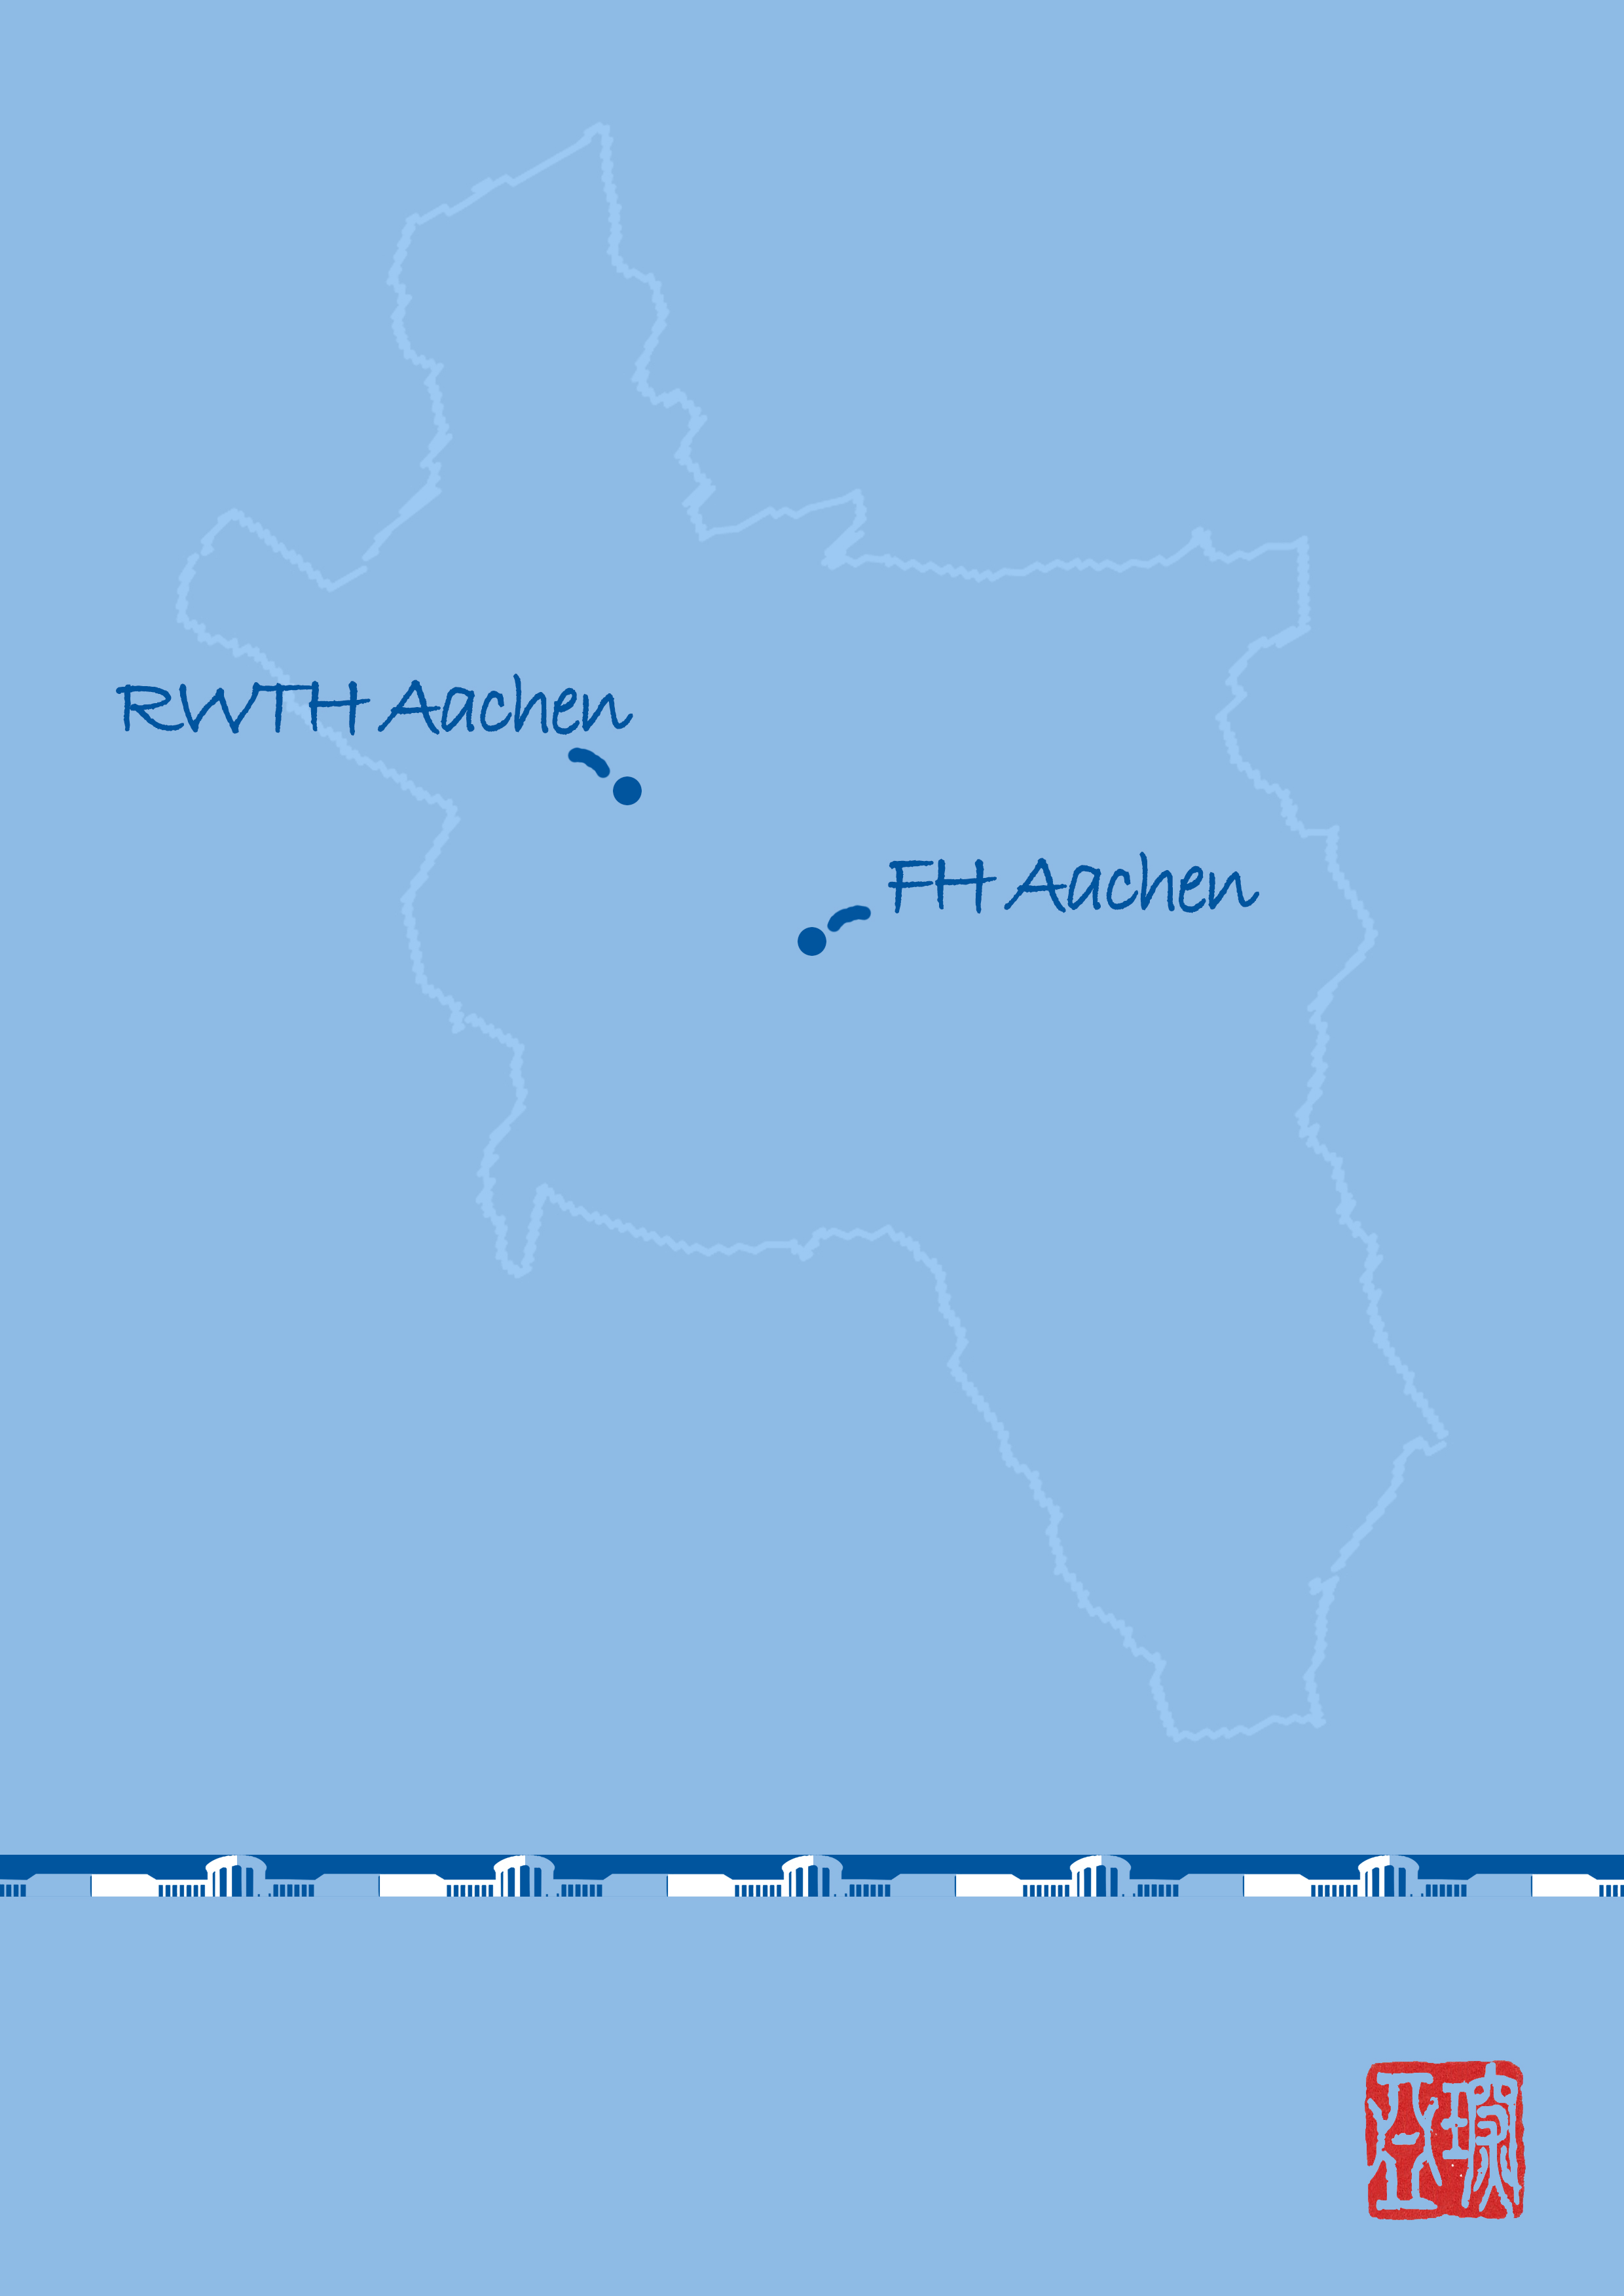
\includegraphics[width=\linewidth]{Bilder/Back_Cover_.jpg}
\end{titlepage}

\end{document}
